\documentclass{llncs}

\usepackage{url}
\usepackage[pdftex]{graphicx}
\usepackage{listings}
\usepackage{verbatim}
\usepackage[lined,linesnumbered,algochapter]{algorithm2e}
\usepackage{tikz}
\usetikzlibrary{arrows,automata}
\usepackage{xspace}
\usepackage {pdfsync}
\usepackage{amsmath}

\usepackage{ngerman}
\usepackage[ngerman, english]{babel}
\usepackage{bibgerm,cite}       % Deutsche Bezeichnungen, Automatisches Zusammenfassen von Literaturstellen
\usepackage[ngerman]{varioref}  % Querverweise

\usepackage{ammalang}

\setcounter{secnumdepth}{2}
\setcounter{tocdepth}{3}

% define custom macros for specific formats or names
\newcommand{\uml}[1]{\texttt{#1}}
\newcommand{\cd}{\textsf{Class Diagram}}

\begin{document}
\pagestyle{plain}
\pagenumbering{roman}

\title{Towards Systematic Mutations for and with ATL Model Transformations\footnote{This work has been created in the context of the course ``188.952 Advanced Model Engineering (VU 2,0)'' in SS15.}}


%&&&&&&&&&&&&&&&&&&&&&&&&&&&&&&&&&&&&&&&&&&&&&&&&&&&&&&&&&&&&&&&&&&&&&&&&
% Name and address of the author
%&&&&&&&&&&&&&&&&&&&&&&&&&&&&&&&&&&&&&&&&&&&&&&&&&&&&&&&&&&&&&&&&&&&&&&&&
\author{Patrick Sommer\inst{1} and Carola Gabriel\inst{2} and Martin Keiblinger\inst{3}}

\institute{Mautner Markhof-Gasse 58/4/31, 1110 Wien \\ \email{e0925011@student.tuwien.ac.at} \\ MatrNr.: 0925011
\and
Mustergasse 54/4/3, 1030 Wien \\ \email{matthias@tuwien.ac.at} \\ MatrNr.: 0426553
\and
Mustergasse 54/4/3, 1030 Wien \\ \email{matthias@tuwien.ac.at} \\ MatrNr.: 0426553
}

\maketitle

\begin{abstract}

Faults in model transformations will produce faults in models. The correction of the defect models are often very expensive. This result affecting the quality of the end product. This is why model transformations have to be correctly tested to maintain product quality. For that mutation testing is a popular technique.  The mutation testing of model transformations have to be developed and for this a suite of mutation operators for the Atlas Transformation language (ATL) are needed. In this paper a set of mutation operators are implemented and the solution of the implementation is discussed and evaluated regarding effectiveness

\end{abstract}

%&&&&&&&&&&&&&&&&&&&&&&&&&&&&&&&&&&&&&&&&&&&&&&&&&&&&&&&&&&&&&&&&&&&&&&&&
% Table of contents
% Activate or deactivate this according to the guideline instructor
%&&&&&&&&&&&&&&&&&&&&&&&&&&&&&&&&&&&&&&&&&&&&&&&&&&&&&&&&&&&&&&&&&&&&&&&&
\tableofcontents
%\thispagestyle{plain}
\newpage

\pagenumbering{arabic}

\section{Introduction}

The broader goal of this work is to create an introduction to a specific field of model driven engineering (MDE). Integral part of MDE is model transformation.\cite{Sendall:2003}. Model transformation allows to synthesize software artifacts from model definitions and ease other software engineering tasks by automating them.

This abstraction eases incremental processes like:\cite{Sendall:2003}
\begin{itemize}
	\item Reverse engineering models e.g. in the process of replacing a legacy system . Then the resulting artifact can be tested and if results of the legacy and the new system are found only the model has to be changed.
	\item Refactoring models
	\item et cetera
\end{itemize}

Therefore the quality of the overall software solution is determined by the quality of the models and the resulting model transformations.\cite{Hutchinson:2011} As a consequence testing the transformations for correctness is a essential part of the quality of the software.\cite{troya:2015}

To check the quality of software is has to be tested. Software testing is a process, or a series processes engineered to check if a program does what it is designed to do and that id does not do anything unintended.\cite{Myers:2004} Model based testing (MBT) is a variant of testing. Test cases are not written by the programmer directly. The programmer creates a model of the requirements and in a second step the test cases are generated on base of the model.\cite{Utting:2012}

Mutation testing or mutation analysis is a fault-based testing technique. It applys changes to the input and creates a mutant. A mutant represents a faulty program. In the best case these changes, which are applied by the mutator, represent mistakes a programmer would make. It has been proven that mutation testing is useful as testing approach but also as:\cite{mutationssurvey:yue}

\begin{enumerate}
	\item Generate input models as test data.
	\item Generate mutants of model transformations.
\end{enumerate}

\subsection{Problem}

To make mutation testing an effective testing method a complete set of mutation operators and a large number of mutated model transformations. Due to the needed size of the sets it's to expensive to create them manually. Additionally the execution of the different models against the test data is a time-consuming.

Therefore automation is required for:

\begin{enumerate}
	\item The generation of a set of mutation operators.
	\item The generation of mutated model transformations.
\end{enumerate}

Furthermore, the computational costs of the executions have to be lowered.

\subsection{Contribution}

Javier et. al. contributed three aspects.

\begin{enumerate}
	\item They have defined a general languagecentric synthesis approach by defining a set of mutation operators based on ATL. 
	\item They made a concept and build a first version of a framework utilizing HOTs for generating mutants.\cite{Paige:2009}
	\item Integrated techniques\cite{Bergmayr:2014} for incremental model transformation execution in their framework.
\end{enumerate}

We contribute further implementations of mutation operators and small tests.

\section{Background}

This work is focused on mutation testing for model transformations. The basic idea of mutation testing in software engineering is not to test the resulting software itself but the test cases.

Good test cases should be able to identify mutants. In he jargon of mutation testing the mutations are \emph{killed}. Killing means recognizing differing results of the original system under test (SUT) and tested mutants.\cite{MatMottu2006}

The process of mutation testing consists of these components:
\begin{itemize}
	\item \textit{Test data} as input for the original programm P and its mutants.
	\item The original program \textit{P}
	\item The \textit{mutants} of P.
	\item An \textit{oracle} which is able to decides if results differ and which is therefore able to identify mutants.
\end{itemize}

The goal of the process\ref{fig:Mutation_Process} is to \textit{kill} or identify faulty versions of P. If a mutant outputs the same data as the P for the same input data it's called \textit{equivalent}. In this case this mutant has to removed from the set of mutants under test.

The last step is to assess how good the tests are and check if they should be improved. Assume \textit{KM} as the set of the killed mutants, \textit{M} is the set of all mutants and \textit{EM} is the set of all identified, equivalent mutants. Then the mutation score \textit{MS} is calculated like this:\cite{mutationssurvey:yue}

\begin{equation}
	MS = \frac{\left|KM\right|}{\left|M\right| - \left|EM\right|}
	\label{eq:ms}
\end{equation}

If this value is to small the tests have to be improved. 

The success of this method depends on the set of mutants used in the process. Manual creation of mutants is a tedious and time consuming task. Therefore a quick, reliable and efficent creation of mutants is proposed in \cite{troya:2015}.

Troya et. al. build upon ATL and higher order transformations (HOT) to create transformations to automatically generate mutants. 

This report show what additional transformation have been developed and what their goal is. The scope of this work is only on the mutation generation in the whole process.

\begin{figure}
	\centering
	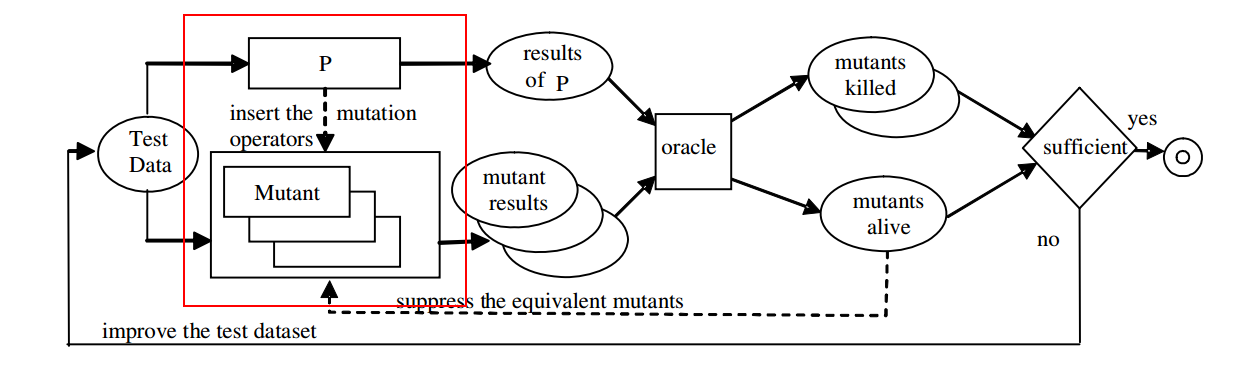
\includegraphics[width=0.7\textwidth]{figures/Marked_Mutation_Process}
	\caption{The mutation testing workflow contains a feedback loop. The red marked area is the part this paper contributes to.\cite{MatMottu2006}}
	\label{fig:Marked_Mutation_Process}
\end{figure}

Model transformations play an important role in the Model Driven Engineering
(MDE) approach. Developing model transformation definitions is expected to
become a common task in model driven software development. \cite{atl:frederic}
In this part of the paper we want to explain the basics of the requirements we needed for Mutations for and with ATL Model Transformations.

\subsection{Model transformation in MDE}

Speaking in broader terms, model transformation is the process of synthesizing one or models from one or more input models. To successfully generate output-models it takes a clear understanding of syntax and semantic of the models and the relationship between their different entities. Model driven engineering provides a formal framework to define this prerequirements.\cite{Sendall:2003}

At the high level exist two categories of model transformations:\cite{Czarnecki03}

\begin{enumerate}
	\item Model to model transformations.
	\item Model to code transformations.
\end{enumerate}

Model to code transformations take models as input and generate source code as output. There exist two different approaches to synthesize the source code. There exists the visitor based approach, which is driven by a model traverse engine which outputs code artifacts when it visits specific points in the model hierarchy. The alternative to the visitor based approach is the template based appraoch. A template consists of constant text and parts which dynamically generate text from the input model. The dynamically part expands iterativly.\cite{Czarnecki03}

There are multiple strategies for model to model transformations:

\begin{itemize}
	\item \emph{Direct-manipulation approache} offers a internal model representation and tools to manipulate it.
	\item The \emph{relational approache} uses relations, in the sense of the mathematical concept, and mapping rules. In combination with a declerative logic, for defining constraints, this is used to produce executable transformations.
	\item The \emph{graph-transformations-based approache} utilizes graph theory, modelling model entities as nodes and edges in the graph, to define model transformations.
	\item The \emph{structure-driven approache} provides the user with a framework to operate on a hierarchy to copy objects and their attributes.
	\item The combination of two or more concepts is called \emph{hybrid approache}.
\end{itemize}

\subsubsection{ATL}

ATL is a model transformation language containing a mixture of declarative and
imperative constructs. ATL is applied in the context of the
transformation pattern shown in \label{fig:overview_atl}. In this pattern a source model Ma is transformed into a target model Mb according to a transformation definition mma2mmb.atl written in the ATL language. The transformation definition is a model conforming to the ATL metamodel. All metamodels conform to the MOF.

\begin{figure}
	\centering
	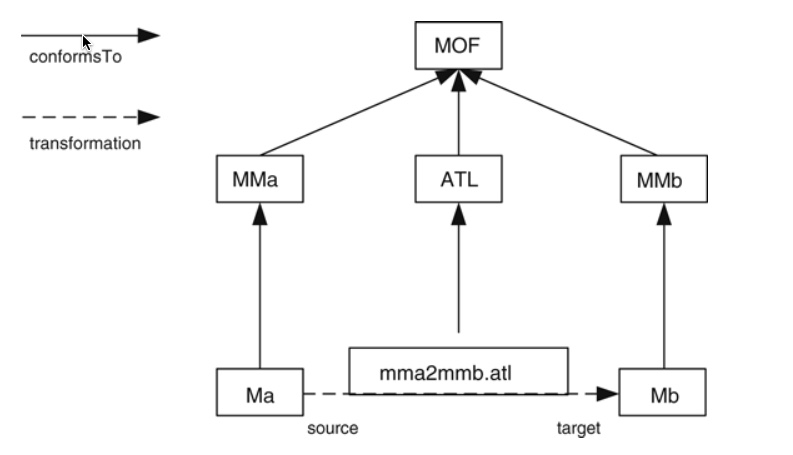
\includegraphics[width=0.7\textwidth,natwidth=610,natheight=642]{figures/Overview_ATL.jpg}
	\caption{Overview of the ATL transformational approach}
	\label{fig:overview_atl}
\end{figure}~\cite{atl:frederic}

ATL is a hybrid transformation language. It contains a mixture of declarative
and imperative constructs. It is encouraged to use a declarative style of specifying transformations. The declarative style of transformation specification has a number of advantages. It is usually based on specifying relations between source and target patterns and thus tends to be closer to the way the developers intuitively perceive a transformation. This style stresses on encoding these relations and hides the details related to selection of source elements, rule triggering and ordering, dealing with traceability, etc. Therefore, it can hide complex transformation algorithms behind a simple syntax.\cite{atl:frederic}

\begin{figure}
	\centering
	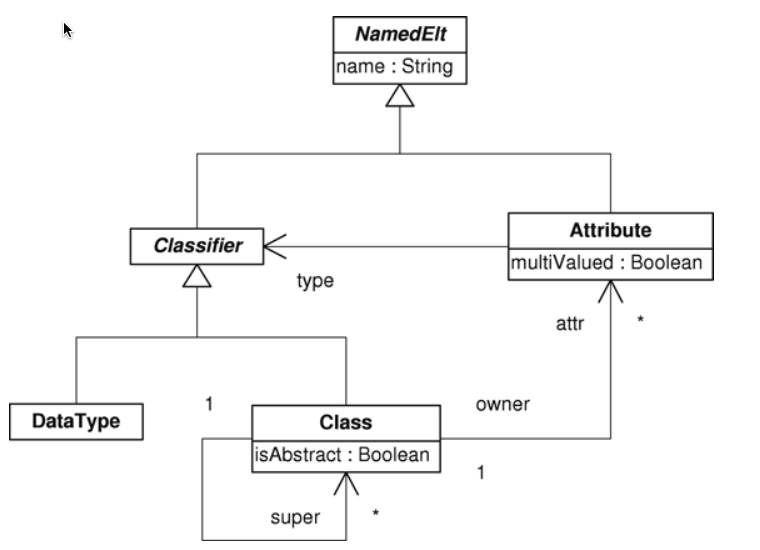
\includegraphics[width=0.7\textwidth,natwidth=610,natheight=642]{figures/Class_metamodel}
	\caption{Class metamodel}
	\label{fig:class_metamodel_atl}
\end{figure}~

The class metamodel is used by the following ATL transformation\ref{lst:shortexample} to create model of the relational metamodel\ref{fig:relational_metamodel_atl}\cite{atl:frederic}

\begin{figure}
	\centering
	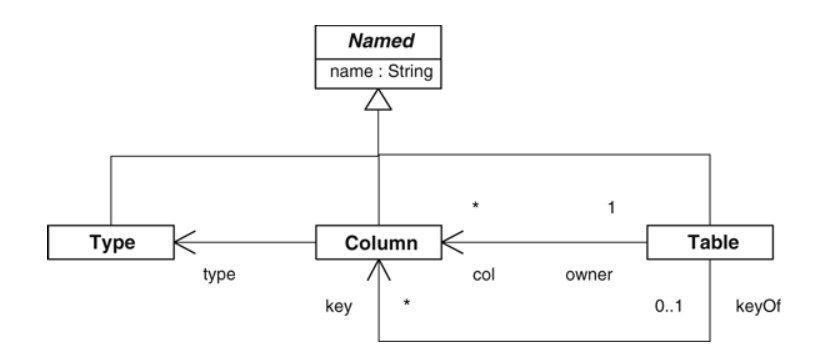
\includegraphics[width=0.7\textwidth,natwidth=610,natheight=642]{figures/Relational_metamodel.jpg}
	\caption{Relational metamodel\cite{atl:frederic}}
	\label{fig:relational_metamodel_atl}
\end{figure}~

\begin{lstlisting}[language=ATL, numbers=left,xleftmargin=5.0ex, caption=Simple example for a ATL transformation, label=lst:shortexample]
//Start Program
module Entities2Forms;
create OUT : Forms from IN : Forms;

rule EntityModel2FormModel {
	from
		em : Forms!EntityModel
	to 
		fm : Forms!FormModel (
			name <- em.name
		)
}
//End Program
\end{lstlisting}

The source model is the 'IN' model and the target model is 'OUT'. The rule mapped the elements EntityModel to FormModel.

\subsubsection{Higher Order Transformations}

Higher order transformations are defined as a model transformation such that
its input and/or output models are themselves transformation models.\cite{Tisi:2009}

In the following figure a sample schema of a HOT for transformation modification
in ATL is shown. The figure show a good overview for the model transformation
such that its input/output models are themselves transformation models.

 \begin{figure}[tb]
	\centering
	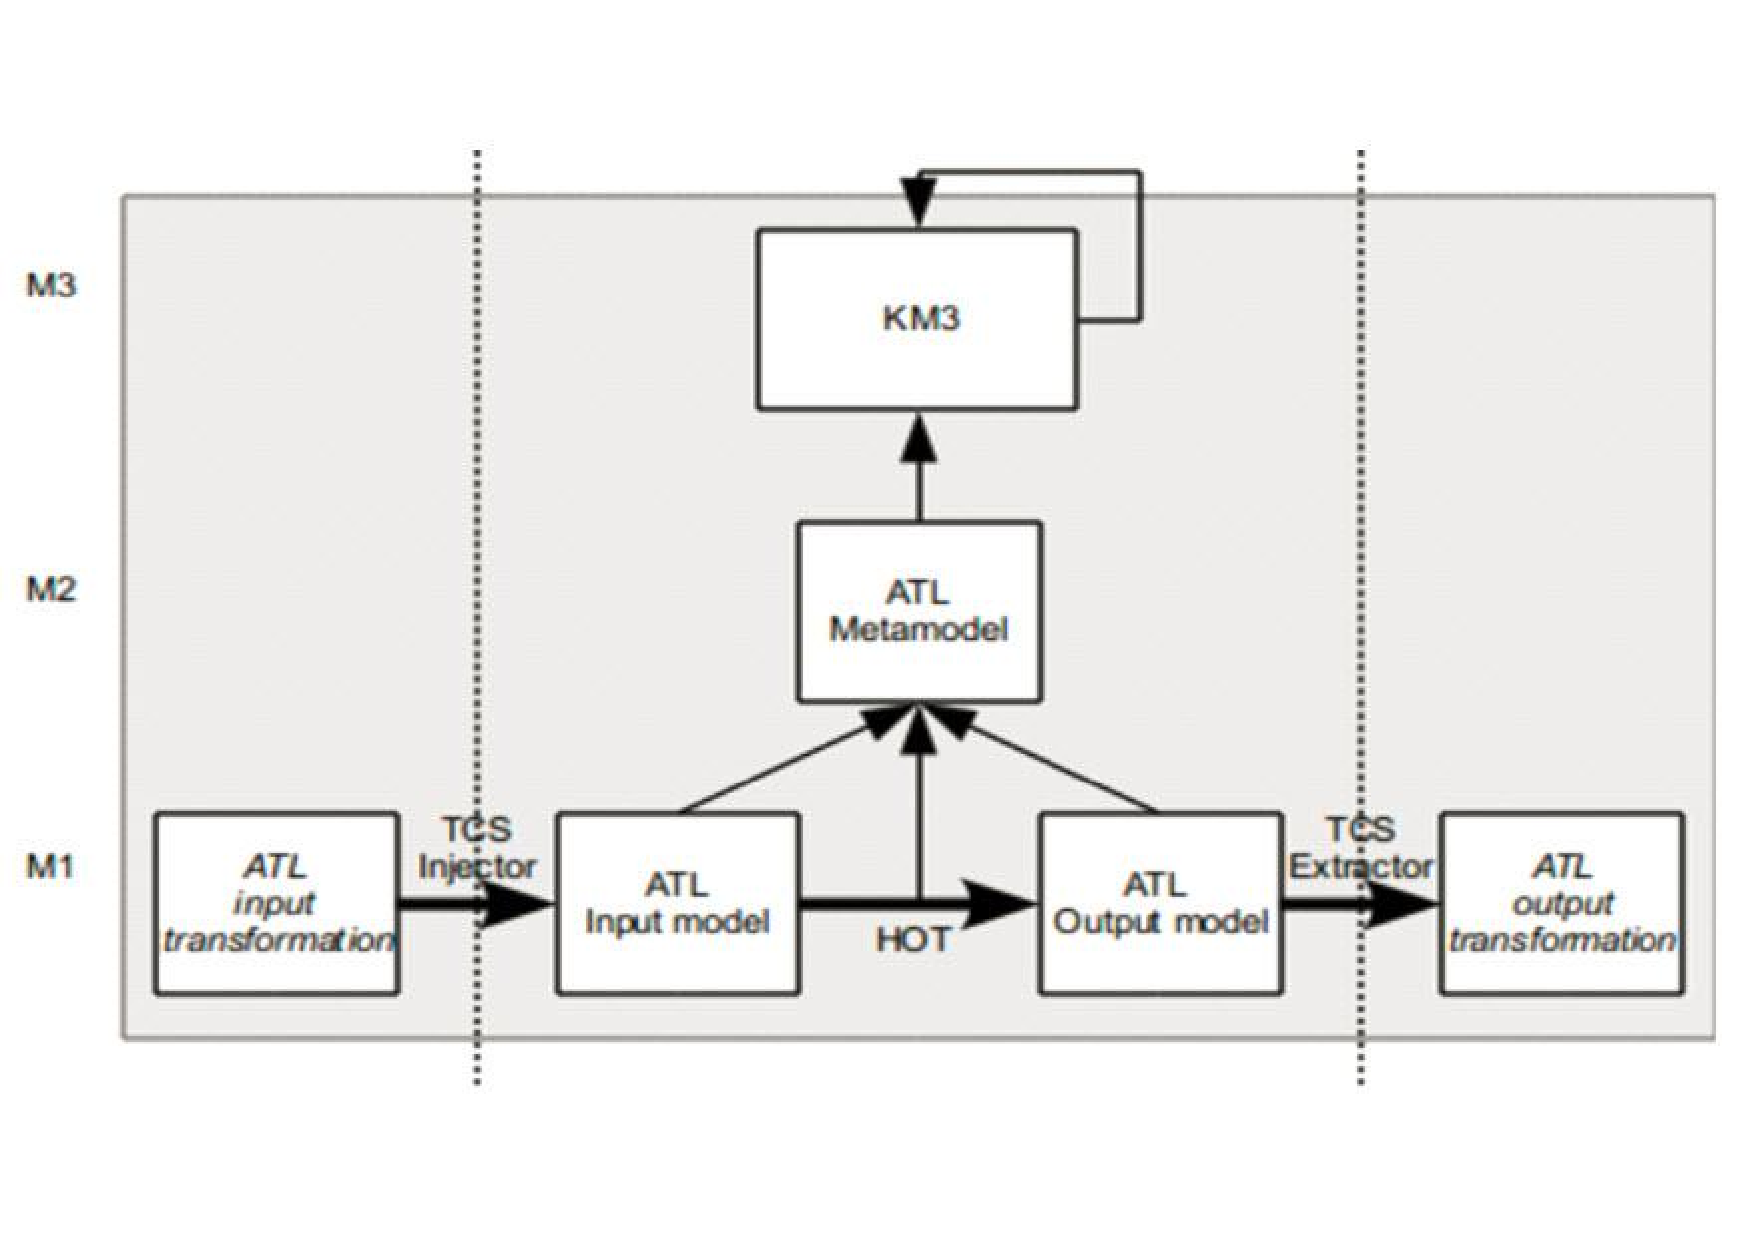
\includegraphics[width=0.7\textwidth,natwidth=610,natheight=642]{figures/HOT.pdf}
	\caption{Sample schema of a HOT for transformation modification in ATL}
	\label{fig:samplefigure_pdf}
\end{figure}~\cite{misc:ModelingLanguages}

Therefore a transformation model is:

\begin{itemize}
	\item The input of a Higher order transformation
	\item The output of a Higher order transformation
	\item Or it is both
\end{itemize}

Tisi et. al identified four transformation patterns for Higher order transformations:

\begin{itemize}
	\item \textbf{Transformation Synthesis} These Higher order transformations generate transformations. If any input is used it's not a transformation.
	\item \textbf{Transformation Analysis} take transformations as input and generate data of different kinds as output. The output is never a transformation.
	\item \textbf{Transformation (De)composition} is the integration of multiple transformations of the input and/or integration of transformations as output.
	\item \textbf{Transformation Modification} is defined by modifing an input transformation and generating an output transformation.
\end{itemize}

The focus of this work is on \textit{Transformation Modifications} (short TM). 

Another possibility of a Higher order transformation is a second Higher order
transformation. That means that a Higher order transformation be also the
input/output of another transformation.

\subsection{Mutations in Model Transformations}
In order to identify the possibility of mutations in languages we have to know
about the concepts of the languages can be mutated. This mutation possibilities
are presented in the referenced paper \cite{troya:2015}. For a better overview
in the following figure there are presented the possible mutations for ATL
transformations.\label{fig:mutations_ATL}

 \begin{figure}[tb]
	\centering
	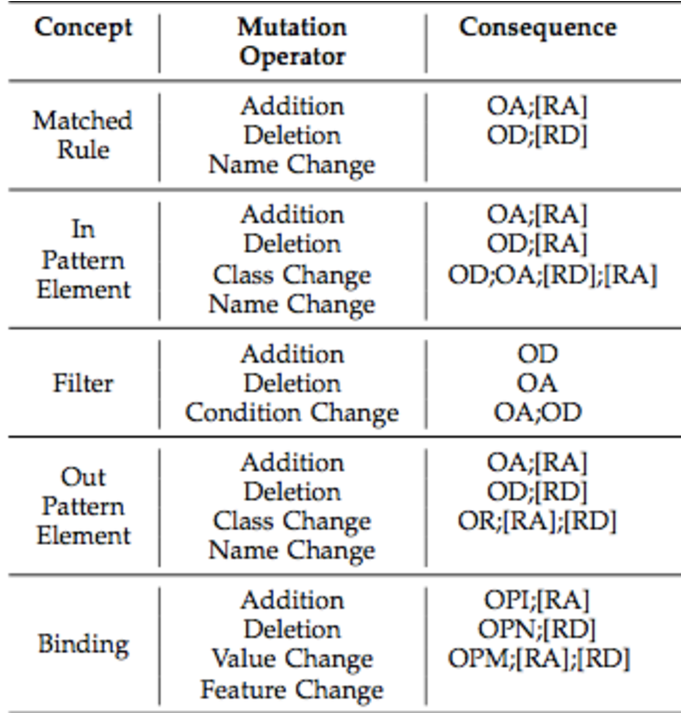
\includegraphics[width=0.7\textwidth,natwidth=610,natheight=642]{figures/Mutations_Identified_for_ATL.pdf}
	\caption{Mutations Identified for ATL transformations}
	\label{fig:mutations_ATL}
\end{figure}~\cite{troya:2015}

In the column \textit{Consequences} of
\label{fig:mutations_ATL} there are some notices about the
consequences of a mutation. In the referenced paper \cite{troya:2015} the
consequences descripted as follows: When a transformation is mutated, it has an effect in the output model that is generated for the same input model as with the original transformation. 

There can be completely new objects that were not present before (OA: Object Addition). Some objects can be deleted (OD: Object Deletion). There can also be
objects that are modified. They are labeled as OPI: Object Property
Initialized or OPN: Object Property set to Null. That means that a property of
an obejct is initialized or is set to null. Another possibility is when the
value of a property of an object is modified (OPM:
Object Property Modified). Or another case is
that an object has replaced (OR: Object Replacement). For OR: Object
Replacement it is important to know that Object Replacemnt can also be seen as
the deletion and addition of an object. The relationships can also be added (RA:
Relationship Added) or deleted (RD: Relationship Deleted).\cite{troya:2015}

For our implemented solutions the consequences OPI: Object Property
Initialized, OPN: Object Property set to Null, OPM:
Object Property Modified, OA: Object
Addition, OR: Object Replacement and OD: Object Deletion are important. In case
of relationships we have to know that the modification of an object implies
automatically the modifictions of relationships and that is why also RA:
Relationship Added or RD: Relationship Deleted are important for our implemented
solutions.

\section{Mutations implemented}

The overall goal of this work is to implement seven transformations. This are defined in \ref{tbl:goals} and show the current status of the work.

\begin{table}[h]
\begin{tabular}{llll}
\textbf{Nr.} & \textbf{Concept}    & \textbf{Mutation operator} & \textbf{Status} \\
1            & Binding             & Value change               & Done            \\
2            & Binding             & Value change               & Done            \\
3            & Binding             & Addition                   &                 \\
4            & Out pattern element & Class change               &                 \\
5            & Out pattern element & Addition                   &                 \\
6            & In pattern element  & Deletion                   & Done            \\
7            & In pattern element  & Class change               &                
\label{tbl:goals}
\end{tabular}
\caption{The implementation goals}
\end{table}

\subsection{Binding}

Bindings are used for the initialization of either \emph{attributes} or \emph{references}. Attributes are primitive values whereas references are relations to other models. Mutation \emph{1} and \emph{2} in table~\ref{tbl:goals} are attribute binding mutations. \emph{3} is a reference binding mutation.

\subsubsection{Deletion}

Deleting a Binding is the implicitly done by omitting the assignment of the attribute or reference in the \emph{to}-part of the ATL rule. The example in listing~\ref{lst:delete} demonstrates the simple structure of delete bindings.

\begin{lstlisting}[language=ATL, numbers=left,xleftmargin=5.0ex, caption=Definition of Delete-Binding., label=lst:delete]
rule DeleteBinding{
  from b: ATL!Binding
  to
}
\end{lstlisting}

\subsubsection{Addition}

\textbf\textit{{Implementation}}

To add a binding is not that easy it seems on the first view.
As we cannot add any binding to an OutPatternElement, we need to know what possible properties the actual class has.
As we don't know this in our High Order Transformation, we have to do a step in between and afterwards do a Second Order HOT to replace the properyName of the binding with an correct propertyName.

As a first step we have to implement our High Order Transformation. To know, where we later have to replace the propertyName, we now set the propertyName to a dummy value like "NewBindingPropertyName".
In Order to have the binding not duplicated, we need to filter our OutPatternElements to only choose the ones wich don't already have the binding with the dummy propertyName.

\begin{lstlisting}[language=ATL, numbers=left,xleftmargin=5.0ex, caption=AddBinding-Definition, label=lst:addbinding]
rule AddBinding{
  from 
  ope : ATL!OutPatternElement ( 
    ope.bindings -> forAll( b | b.propertyName <> 'NewBinding_PropertyName')
  )
  to
  ope2 : ATL!OutPatternElement (
    bindings <- ope.bindings -> append(bindingNewElement)
  ), 
  bindingNewElement : ATL!Binding (
    outPatternElement <- ope2,
    propertyName <- 'NewBinding_PropertyName',
    value <- newValue	
  ),
  newValue : ATL!StringExp (
    stringSymbol <- 'testvalue'
  )	
}
\end{lstlisting}

This dummy value will be replaced in the Second Order HOT.
We search in our ATL Metamodel for all StringExpressions with our dummy value and replace it with a new value.
To get this new value we search for our general supertype in our metamodel. From this supertype we can now choose an attribute (called EStructuralFeature), which we can add to all of the subtypes.

\begin{lstlisting}[language=ATL, numbers=left,xleftmargin=5.0ex, caption=AddBindingNames-Definition., label=lst:addbindingnames]
rule AddBindingNames {
from b : ATL!StringExp (
    b.stringSymbol = 'NewBinding_PropertyName'
)
using{
  classes : Sequence(OUT_MM!EClass) 
	= OUT_MM!EClass.allInstancesFrom('OUT_MM') 
	-> select(c | c.getESuperTypes() -> size() <= 0);
}
to b2 : ATL!StringExp ( 
  stringSymbol <- classes 
	-> first().getEStructuralFeatures() -> last().name
)	
}
\end{lstlisting}

There are two types of major types of binding values in the ATL metamodel:

\begin{itemize}
	\item Primitive Expressions
	\item Variable Expressions
\end{itemize}

The primitive expressions are directly assignable in the ATL rules. Variable expressions have to be composed from the available objects in the metamodel. (See \ref{fig:atl_mm_excerpt})

\begin{figure}
	\centering
	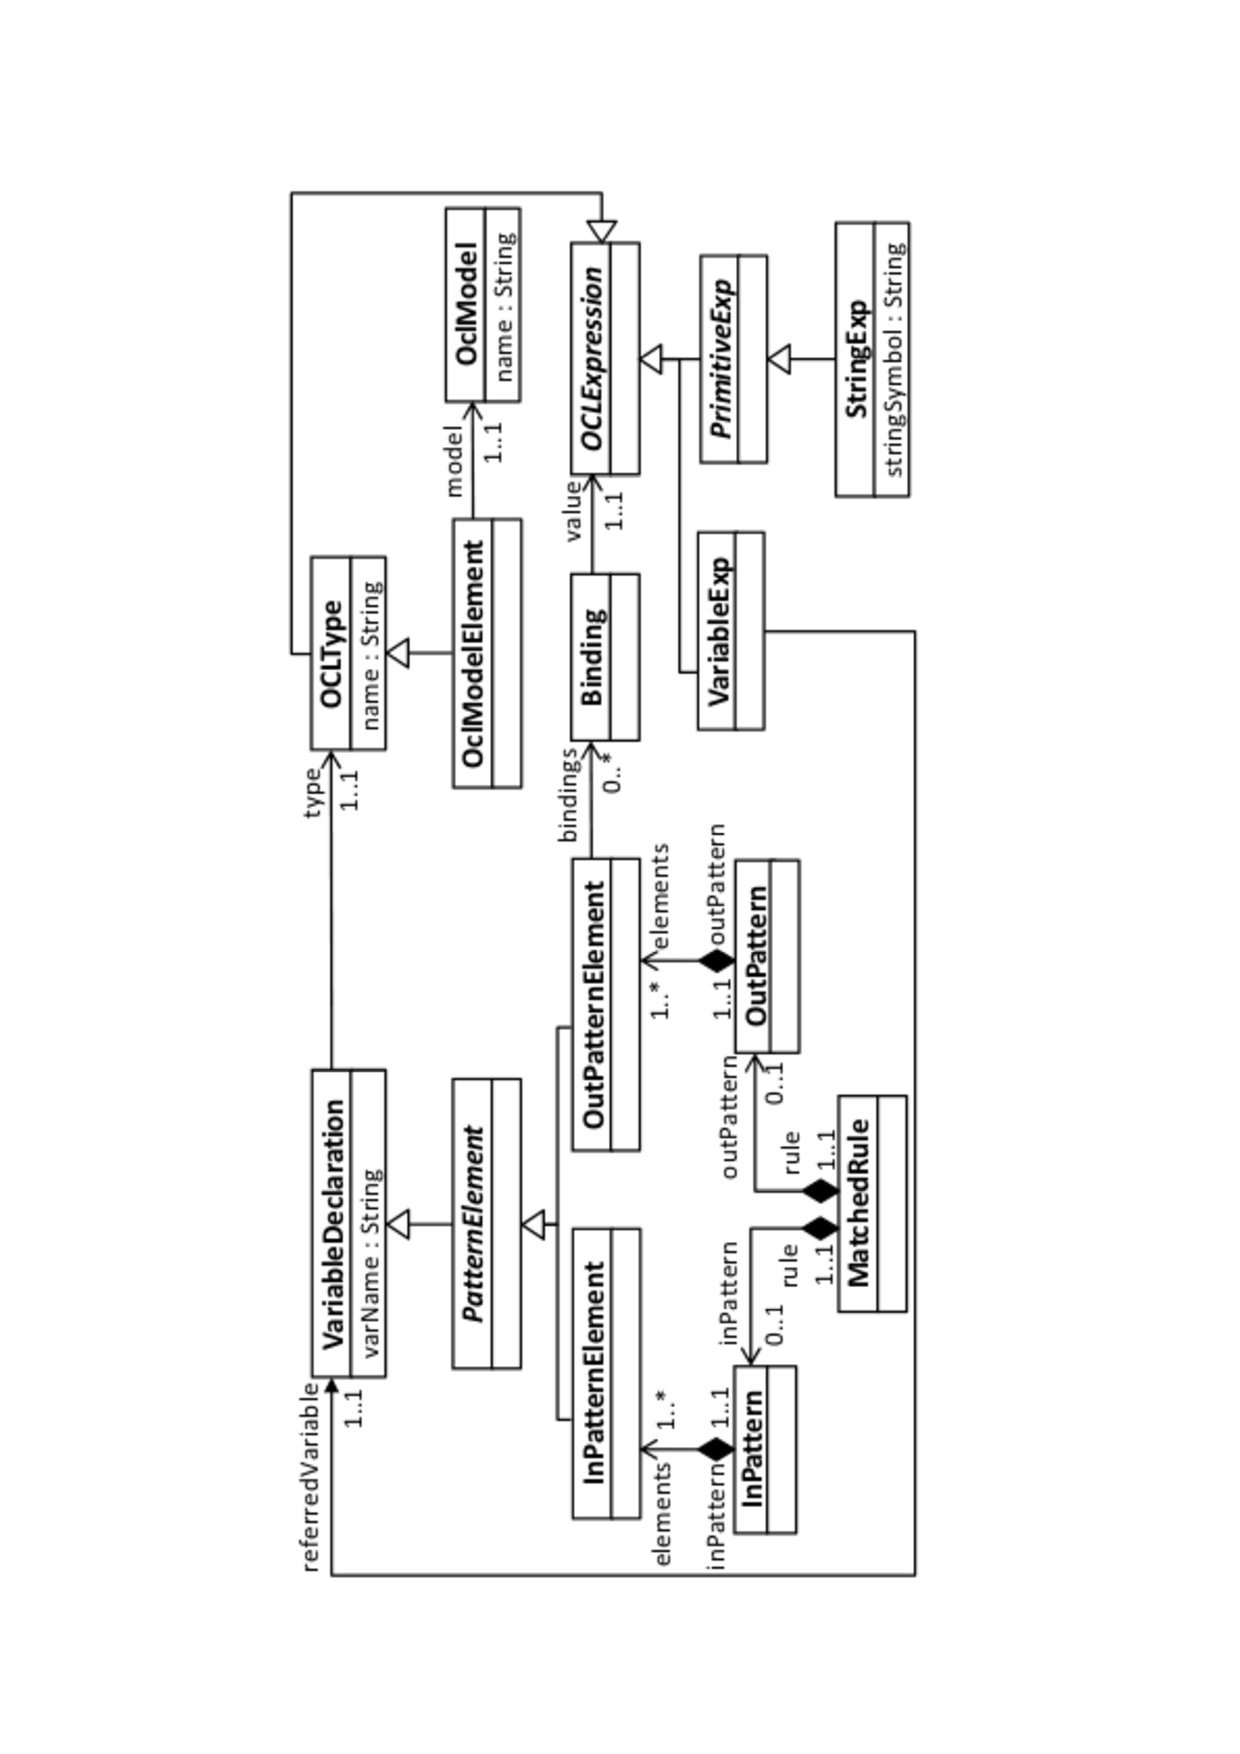
\includegraphics[width=0.7\textwidth,natwidth=610,natheight=642]{figures/ATL_Metamodel_Excerpt}
	\caption{Excerpt of the ATL metamodel}
	\label{fig:atl_metamodel_excerpt}
\end{figure}~

The first example shows how to change the value of all String Expressions. The output value will be the String "Hello".

To achieve this, we first have to search for all bindings with the value type "ATL!StringExp" and set this value to our defined string value.

\begin{lstlisting}[language=ATL, numbers=left,xleftmargin=5.0ex, caption=ValueChangeBinding-Definition., label=lst:valuechangebinding]
rule ValueChangeBinding_All{
	from
	 b : ATL!Binding (b.value.oclIsTypeOf(ATL!StringExp))
	to
	 c : ATL!Binding (
	 	value <- newStringExp
	 ),
	 newStringExp : ATL!StringExp(
	 	stringSymbol <- 'hello'	
	 )
}
\end{lstlisting}

As an extension to this approach, in a second step we want to overwrite all String expressions to the first String value of the input model. This only make sense, if we have more than one string expression, so we added a condition to do this.

\begin{lstlisting}[language=ATL, numbers=left,xleftmargin=5.0ex, caption=ValueChangeBinding-Definition using same constant string value., label=lst:vcbconstant]
rule ValueChangeBinding_AllSameStringValue{
	from
	 b : ATL!Binding(
	 	b.value.oclIsTypeOf(ATL!StringExp) and 
		ATL!StringExp.allInstances() -> size() > 1
	 )
	to
	 c : ATL!Binding(
	 	value <- stringexpression
	 ), 
	 stringexpression : ATL!StringExp(
	 	stringSymbol <- (ATL!StringExp.allInstances() 
			-> first()).stringSymbol
	)
\end{lstlisting}

The third approach in this category was to switch the first with the last value binding. For this we fist filter only the OutPatternElements which have more than one binding and have only StringExpression bindings.

As a second step we exclude the first and the last binding from the binding-list to replace them with our new bindings with the prepend and append commands. As a third step we have to create our new binding-elements.

Such a binding element needs three values: the corresponding OutPatternElement, the property name and the value.

As outPatternElement and propertyName we take the original outPatternElement and propertyName, as value, we take value from the last binding for our new first elemen and the value from the fist binding for our new last element.

Important to achieve correct values is, that we use the original binding list from the "from"-clause of the rule.

\begin{lstlisting}[language=ATL, numbers=left,xleftmargin=5.0ex, caption=ValueChangeBinding-Definition using values from input models., label=lst:2ndOrderHOT]
rule ValueChangeBinding_Switch{
from
ope : ATL!OutPatternElement (
	ope.bindings 
		-> forAll(e | e.value.oclIsTypeOf(ATL!StringExp)) and
		ope.bindings -> size() > 1
)
to
ope2 : ATL!OutPatternElement (
	bindings <- ope.bindings -> excluding (ope.bindings -> first()) 
		-> excluding (ope.bindings -> last())
		-> prepend (bindingNewFirst)
		-> append (bindingNewLast)
), 
bindingNewLast : ATL!Binding (
	outPatternElement <- ope2, 
	propertyName <- (ope.bindings -> last()).propertyName,
	value <- (ope.bindings -> first()).value
),
bindingNewFirst : ATL!Binding (
	outPatternElement <- ope2,
	propertyName <- (ope.bindings -> first()).propertyName,
	value <- (ope.bindings -> last()).value	
)
	
}
\end{lstlisting}

\subsubsection{Deletion}

To delete an InPatternElement it is not enough to delete only the InPatternElement itself. You have to deal at least with one important effect. The usage of this InPatternElement in the Bindings of the OutPatternElements.

For better understanding this problem, I will give a short example.

\begin{lstlisting}[language=ATL, numbers=left,xleftmargin=5.0ex]
rule PNMLDocument {
	from
		e : PetriNet!PetriNet,
		f : PetriNet!PetriNet
	to	
		n : PNML!PNMLDocument
		(
			location <- e.location,
			xmlns <- uri,
			nets <- net			
		)
\end{lstlisting}

\begin{lstlisting}[language=ATL, numbers=left,xleftmargin=5.0ex]
rule PNMLDocument {
	from
		f : PetriNet!PetriNet
	to	
		n : PNML!PNMLDocument
		(
			location <- .location,
			xmlns <- uri,
			nets <- net			
		)
\end{lstlisting}

If you delete the IPE with the variableName e, the binding location <- e.location will have an unreferredVariable in its value part. So the generated model is not valid any more. To avoid this, you have to delete all bindings with unreferred variables in a second step of your high order transformations.

The implementation of the deletion of an IPE looks like this:
\begin{lstlisting}[language=ATL, numbers=left,xleftmargin=5.0ex]
rule DelteIPE {
  from ipe : ATL!InPatternElement (
    ipe.inPattern.elements -> size() > 1 and
    ipe = ipe.inPattern.elements -> last()
  )
\end{lstlisting}

The following deletion of Binding is realized with this code:
\begin{lstlisting}[language=ATL, numbers=left,xleftmargin=5.0ex]
rule DelteNavigationBinding{
from b : ATL!Binding(
	b.value.oclIsTypeOf(ATL!NavigationOrAttributeCallExp) and 
	b.value.source.referredVariable.oclIsUndefined()
)
to
}
rule DeleteCollectionBinding{
from b:ATL!Binding(		
	b.value.oclIsTypeOf(ATL!CollectionOperationCallExp) and 
	b.value.source.oclIsTypeOf(ATL!NavigationOrAttributeCallExp) and 
	b.value.source.source.referredVariable.oclIsUndefined()
)
to
}
\end{lstlisting}

First of all you need to know, that there are several types of possible binding values - the CollectionOperationCallExp and the NavigationOrAttributeCallExp.
As they have a different strucutre and to deal with both of them. you have to write two rules to delete the corresponding bindings.

\section{Related work}
In the related work \cite{troya:2015} the authors have identified the mutations for ATL transformation language as in chapter \textit{Mutations in Model Transformations} descripted. We have implemented a set of possible mutations in AATl they have identified. For the general part of the paper we have read some other papers with different approaches.

\section{Conclusion and future work}
In this paper we have implemented some solutions regarding mutations in ATL. The implementation of a set of mutation operators is discussed and evaluated regarding effectiveness. We have selected some mutations in ATL like Binding (Addtion, Deletion and Change), In Pattern Element (Addition, Class change) and Out Pattern Element (Deletion, Class change). In the paper we have explain the effect of the mutations of transformtions and we see that there are many consequences. The approach presented in this paper aims at mutation of model transformations for building trust into model transformation programs using this technique. Further work will consist in deveolpment of tools for autmated mutations of model transformations. First only for ATL and second for other model transformation languages for example like QVT.

\section{Bibliographic Issues}

\subsection{Literature Search}

Information on online libraries and literature search, e.g., interesting magazines, journals, conferences, and organizations may be found at \url{http://www.big.tuwien.ac.at/teaching/info.html}.

\subsection{BibTeX}

BibTeX should be used for referencing.

The LaTeX source document of this pdf document provides you with different samples for references to journals~\cite{jour:B2BServices}, conference papers~\cite{proc:TheWebMLApproach}, books~\cite{book:umlatwork}, book chapters~\cite{incoll:ErhardKonrad1992}, electronic standards~\cite{man:BPEL}, dissertations~\cite{phdthesis:manuelWimmer}, masters' theses~\cite{mast:AUMLProfile}, and web sites~\cite{misc:BIGWebsite}. The respective BibTeX entries may be found in the file \texttt{references.bib}. For administration of the BibTeX references we recommend \url{http://www.citeulike.org} or JabRef for offline administration, respectively.

\bibliographystyle{acm}
\bibliography{references}

\end{document}
